\section{Drawing Stuff}

There are several powerful packages (such as \texttt{pgfplots} \ref{sec:pgfplots} and \texttt{tikz} \ref{sec:tikz}) which allow for drawing plots and graphs directly in your \LaTeX{} document.
It be noted how they may noticeably increase compile times. % https://www.overleaf.com/learn/latex/Questions/I_have_a_lot_of_tikz%2C_matlab2tikz_or_pgfplots_figures%2C_so_I%27m_getting_a_compilation_timeout._Can_I_externalise_my_figures%3F

\subsection{With \texttt{pgfplots}}\label{sec:pgfplots}

Some nice graphs can be drawn using the \texttt{pgfplots} package.

% Demonstrate graphing of functions - https://www.overleaf.com/learn/latex/Pgfplots_package
\begin{figure}[H]
	\centering
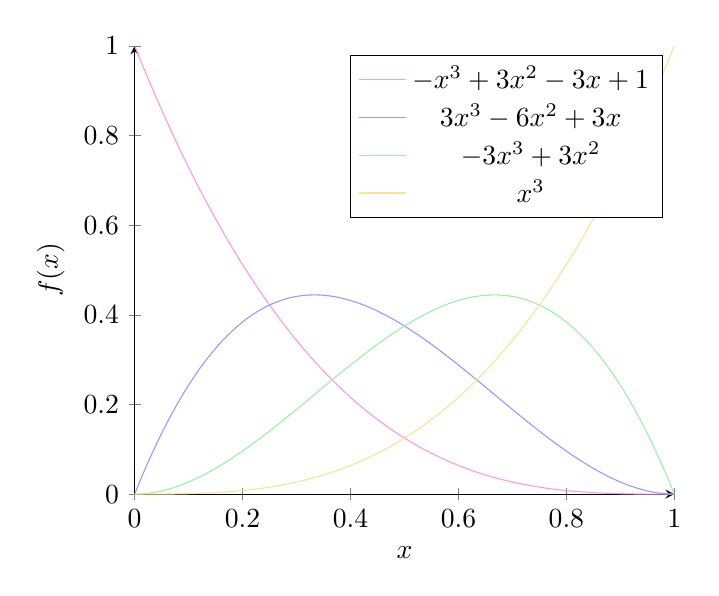
\begin{tikzpicture}\begin{axis}[
	axis lines = left,
	xlabel = {$x$},
	ylabel = {$f(x)$},
]
%	\addplot[
%		domain=-4:3,
%		samples=100,
%		color=red,
%	]{
%		x^2 - 2*x - 1
%	};
%	\addlegendentry{$x^2 - 2x - 1$}
%	
%	\addplot[
%		domain=-4:3,
%		samples=100,
%		color=blue,
%	]{
%		x^3 / (2^(-x) + 1)
%	};
%	\addlegendentry{$\frac{x^3}{2^{-x} + 1}$}

	\addplot[
		domain=0:1,
		samples=100,
		color=red!25!magenta!40!white,
	]{
		-x^3 + 3*x^2 - 3*x + 1
	};
	\addlegendentry{$-x^3+3x^2-3x+1$}

	\addplot[
		domain=0:1,
		samples=100,
		color=blue!100!cyan!40!white,
	]{
		3*x^3 - 6*x^2 + 3*x
	};
	\addlegendentry{$3x^3 - 6x^2 + 3x$}

	\addplot[
		domain=0:1,
		samples=100,
		color=green!75!teal!40!white,
	]{
		-3*x^3 + 3*x^2
	};
	\addlegendentry{$-3x^3 + 3x^2$}

	\addplot[
		domain=0:1,
		samples=100,
		color=yellow!50!orange!40!white,
	]{
		x^3
	};
	\addlegendentry{$x^3$}
\end{axis}\end{tikzpicture}
	\caption{2D example of Bernstein polynomials.}
	\label{fig:fungraph}
\end{figure}

\begin{figure}[H]
	\centering
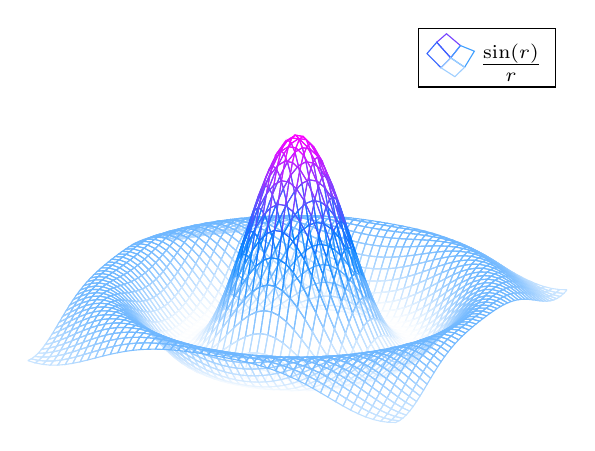
\begin{tikzpicture}\begin{axis}[
	hide axis,
	colormap/cool,
]
	\addplot3[
		mesh,
		samples=50,
		domain=-8:8,
	]{
		sin(deg(sqrt(x^2+y^2)))/sqrt(x^2+y^2)
	};
	\addlegendentry{$\frac{\sin(r)}{r}$}
\end{axis}\end{tikzpicture}
	\caption{3D example, using the mesh parameter.}
	\label{fig:meshgraph}
\end{figure}

\subsection{With \texttt{tikz}}\label{sec:tikz}

Here are some graphs drawn using Ti\textit{k}Z.
Doing this can sometimes be a little \emoji{painful} (painfully time-consuming) in my opinion, but the resulting vector graphics are quite timeless.

% Demonstrate drawing of graphs - https://www.baeldung.com/cs/latex-drawing-graphs
\begin{figure}
	\centering
	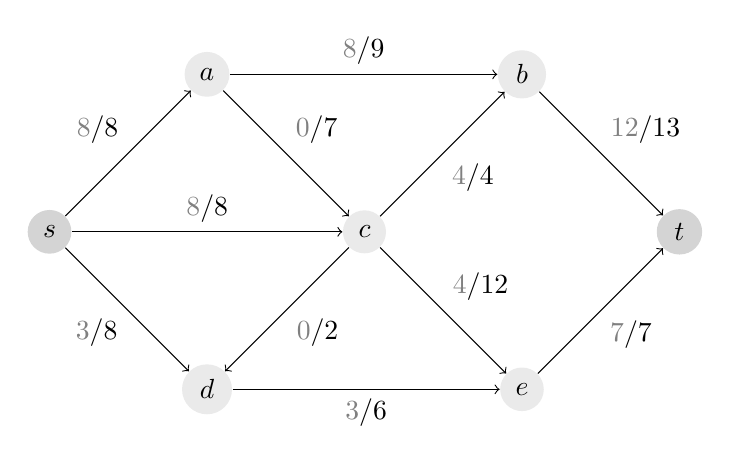
\begin{tikzpicture}[default/.style={circle, fill=lightgray!33}]
%	\node[rectangle, draw] at (-1,2.5) (mylabel) {$N$ under $f^{++}$};
	\node[default, fill=lightgray!67] at (0,0) (s) {$s$};
	\node[default] at (2,2) (a) {$a$};
	\node[default] at (6,2) (b) {$b$};
	\node[default] at (4,0) (c) {$c$};
	\node[default] at (2,-2) (d) {$d$};
	\node[default] at (6,-2) (e) {$e$};
	\node[default, fill=lightgray!67] at (8,0) (t) {$t$};

	\draw[->] (s) edge node[midway, anchor=south east]{$\textcolor{gray}{8}/8$} (a);
	\draw[->] (s) edge node[midway, anchor=south]{$\textcolor{gray}{8}/8$} (c);
	\draw[->] (s) edge node[midway, anchor=north east]{$\textcolor{gray}{3}/8$} (d);
	\draw[->] (a) edge node[midway, anchor=south]{$\textcolor{gray}{8}/9$} (b);
	\draw[->] (a) edge node[midway, anchor=south west]{$\textcolor{gray}{0}/7$} (c);
	\draw[->] (b) edge node[midway, anchor=south west]{$\textcolor{gray}{12}/13$} (t);
	\draw[->] (c) edge node[midway, anchor=north west]{$\textcolor{gray}{4}/4$} (b);
	\draw[->] (c) edge node[midway, anchor=north west]{$\textcolor{gray}{0}/2$} (d);
	\draw[->] (c) edge node[midway, anchor=south west]{$\textcolor{gray}{4}/12$} (e);
	\draw[->] (d) edge node[midway, anchor=north]{$\textcolor{gray}{3}/6$} (e);
	\draw[->] (e) edge node[midway, anchor=north west]{$\textcolor{gray}{7}/7$} (t);
	\end{tikzpicture}
	\caption{Graph for a flow network $N$.}
	\label{fig:N}
\end{figure}

\begin{figure}
	\centering
	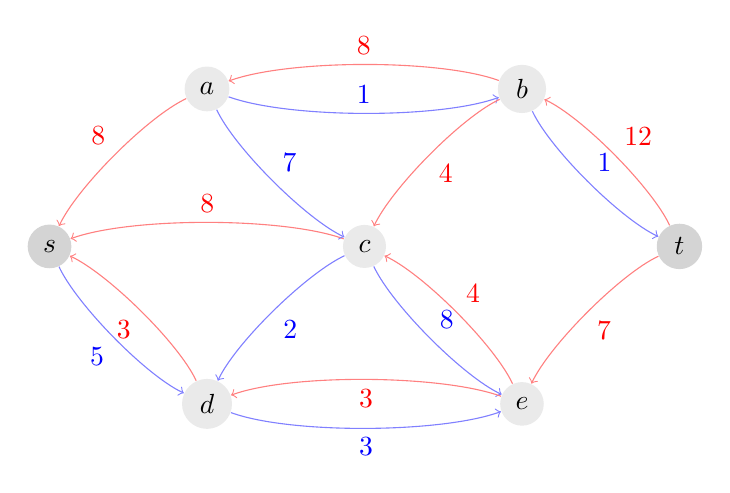
\begin{tikzpicture}[default/.style={circle, fill=lightgray!33}]
%	\node[rectangle, draw] at (-1,2.5) (mylabel) {$N_{f^{++}}$};
	\node[default, fill=lightgray!67] at (0,0) (s) {$s$};
	\node[default] at (2,2) (a) {$a$};
	\node[default] at (6,2) (b) {$b$};
	\node[default] at (4,0) (c) {$c$};
	\node[default] at (2,-2) (d) {$d$};
	\node[default] at (6,-2) (e) {$e$};
	\node[default, fill=lightgray!67] at (8,0) (t) {$t$};
	
	\draw[->] (a) edge[red!50, out=205,in=65,looseness=0.6] node[midway, anchor=south east]{$\textcolor{red}{8}$} (s);
	\draw[->] (c) edge[red!50, out=160,in=20,looseness=0.6] node[midway, anchor=south]{$\textcolor{red}{8}$} (s);
	\draw[->] (s) edge[blue!50, out=295,in=155,looseness=0.6] node[midway, anchor=north east]{$\textcolor{blue}{5}$} (d);
	\draw[->] (d) edge[red!50, out=115,in=335,looseness=0.6] node[midway, anchor=north east]{$\textcolor{red}{3}$} (s);
	\draw[->] (a) edge[blue!50, out=340,in=200,looseness=0.6] node[midway, anchor=south]{$\textcolor{blue}{1}$} (b);
	\draw[->] (b) edge[red!50, out=160,in=20,looseness=0.6] node[midway, anchor=south]{$\textcolor{red}{8}$} (a);
	\draw[->] (a) edge[blue!50, out=295,in=155,looseness=0.6] node[midway, anchor=south west]{$\textcolor{blue}{7}$} (c);
	\draw[->] (b) edge[blue!50, out=295,in=155,looseness=0.6] node[midway, anchor=south west]{$\textcolor{blue}{1}$} (t);
	\draw[->] (t) edge[red!50, out=115,in=335,looseness=0.6] node[midway, anchor=south west]{$\textcolor{red}{12}$} (b);
	\draw[->] (b) edge[red!50, out=205,in=65,looseness=0.6] node[midway, anchor=north west]{$\textcolor{red}{4}$} (c);
	\draw[->] (c) edge[blue!50, out=205,in=65,looseness=0.6] node[midway, anchor=north west]{$\textcolor{blue}{2}$} (d);
	\draw[->] (c) edge[blue!50, out=295,in=155,looseness=0.6] node[midway, anchor=south west]{$\textcolor{blue}{8}$} (e);
	\draw[->] (e) edge[red!50, out=115,in=335,looseness=0.6] node[midway, anchor=south west]{$\textcolor{red}{4}$} (c);
	\draw[->] (d) edge[blue!50, out=340,in=200,looseness=0.6] node[midway, anchor=north]{$\textcolor{blue}{3}$} (e);
	\draw[->] (e) edge[red!50, out=160,in=20,looseness=0.6] node[midway, anchor=north]{$\textcolor{red}{3}$} (d);
	\draw[->] (t) edge[red!50, out=205,in=65,looseness=0.6] node[midway, anchor=north west]{$\textcolor{red}{7}$} (e);
	\end{tikzpicture}
	\caption{Residue graph for the network $N$.}
	\label{fig:Nres}
\end{figure}

\begin{figure}
	\centering
	\begin{tikzpicture}[lbl/.style={circle,fill=pagecol,midway,anchor=center}]
%	\node[rectangle, draw] at (-1,2.5) (mylabel) {$N$ with $(S,T)$};
	\node[circle,fill=cyan!25] at (0,0) (s) {$s$};
	\node[circle,fill=orange!25] at (2,2) (a) {$a$};
	\node[circle,fill=orange!25] at (6,2) (b) {$b$};
	\node[circle,fill=cyan!25] at (4,0) (c) {$c$};
	\node[circle,fill=cyan!25] at (2,-2) (d) {$d$};
	\node[circle,fill=cyan!25] at (6,-2) (e) {$e$};
	\node[circle,fill=orange!25] at (8,0) (t) {$t$};

	\draw[->] (s) edge node[lbl]{$8$} (a);
	\draw[->] (s) edge[lightgray] (c);
	\draw[->] (s) edge[lightgray] (d);
	\draw[->] (a) edge[lightgray] (b);
	\draw[->] (a) edge[lightgray] (c);
	\draw[->] (b) edge[lightgray] (t);
	\draw[->] (c) edge node[lbl]{$4$} (b);
	\draw[->] (c) edge[lightgray] (d);
	\draw[->] (c) edge[lightgray] (e);
	\draw[->] (d) edge[lightgray] (e);
	\draw[->] (e) edge node[lbl]{$7$} (t);
	\end{tikzpicture}
	\caption{An $s$-$t$-cut for network $N$.}
	\label{fig:Ncut}
\end{figure}

\subsection{With \texttt{tcolorbox}}

--- \textit{``These colorboxes are pretty nifty, thanks \href{https://www.ctan.org/pkg/tcolorbox}{Dr.Dr.Sturm!}''}

What follow are some examples with placeholder text inbetween.

\bigskip
% Add an 'algorithm' box
\begin{lalg}{Depth First Search}
	We could implement an iterative version of depth first search as follows
% Typeset some code
% Use custom style defined in preamble
% Optionally specify language syntax highlighting
% Allows escaping math (with this style)
	\begin{lstlisting}[style=L,language=Python]
# The runtime of DFS is in $\On(|V|+|E|)$.
# PRE : `graph` has method `neighbors_of(node)`
def depth_first_search(graph, start_node): 
	stack   = [start_node]
	visited = {start_node}
	while stack:
		current = stack.pop()
		for neighbor in graph.neighbors_of(current):
			if neighbor not in visited:
				stack.append(neighbor)
				visited.add(neighbor)
	\end{lstlisting}
\end{lalg}

\bigskip
\textit{I like this player. It played well. It did not give up.}
\bigskip

% Use a customized tcolorbox - https://xyquadrat.ch/2022/04/04/latex-boxes/
\marginpar{\raggedright Notable thanks to \href{https://xyquadrat.ch/2022/04/04/latex-boxes/}{xyquadrat}}
\begin{tcolorbox}[
	adjusted title=Equivalence Relation, fonttitle=\bfseries,
	boxrule=0mm, leftrule=1mm, arc=0mm, 
	left=1.75mm, toptitle=0.75mm, bottomtitle=0.25mm,
	colframe=brandblue,
	coltitle=textcol, colbacktitle=textcol!10!pagecol,
	coltext=textcol, colback=textcol!5!pagecol,
]
	\def\EAx<#1>{E#1)}
	Given some set $A$ and the relation $\rho\subseteq A\times A$.
	We call $\rho$ an equivalence relation on $A$ if it fulfils the three axioms \EAx<1> - \EAx<3>
% Demonstrate custom enumeration
	\begin{enumerate}[label=\EAx<\arabic*>]
		\item Reflexivity, $\id\subseteq\rho \iff \forall a\in A: a\,\rho\,a$.
		\item Symmetry, $\rho=\hat\rho \iff \forall a,b\in A: a\,\rho\,b \leftrightarrow b\,\rho\,a$.
		\item Transitivity, $\rho^2\subseteq\rho \iff \forall a,b,c\in A: a\,\rho\,b \land b\,\rho\,c \rightarrow a\,\rho\,c$.
	\end{enumerate}
	We call $\rho$ an order relation (or partial order) on $A$ if it fulfils axioms \EAx<1>, \EAx<3> and \EAx<4>.
% 'Continue' enumeration
	\begin{enumerate}[label=\EAx<\arabic*>]\setcounter{enumi}{3}
		\item Antisymmetry, $\rho\cap\hat\rho\subseteq\id \iff \forall a,b\in A: a\,\rho\,b \land b\,\rho\,a \rightarrow b=a$.
	\end{enumerate}
\end{tcolorbox}

\bigskip
\textit{This player dreamed of sunlight and trees. Of fire and water. It dreamed it created. And it dreamed it destroyed. It dreamed it hunted, and was hunted. It dreamed of shelter.}
\bigskip

% Demonstrate tcolorbox with image
\begin{tcolorbox}[
	enhanced,
	adjusted title=\textbf{Binomial Coefficient},
	frame style image=ETH.jpg,
	opacityback=0.80, opacitybacktitle=0.20,
	colback=blue!5!white, colframe=blue!75!black,
]
	The Binomial Coefficient is the coefficient of the $x^k$ term in the polynomial expansion of the binomial power $(1+x)^n$. % % https://en.wikipedia.org/wiki/Binomial_coefficient
	It can be compactly expressed as
	\[ \phantom{1}_nC_k = \prod_{i=1}^k \frac{n+1-i}{i} = \frac{n!}{k!(n-k)!} = \binom{n}{k} \]
	which is usually read as "$n$ choose $k$".
	The coefficient determines the number of ways to choose an unordered subset of $k$ items from a fixed set of $n$ elements.
	It satisfies the recurrence relation $\binom{n}{k} = \binom{n-1}{k-1} + \binom{n-1}{k}$. % https://en.wikipedia.org/wiki/Pascal%27s_triangle
\end{tcolorbox}

\bigskip
\textit{Sometimes the player dreamed it was other things, in other places. Sometimes these dreams were disturbing. Sometimes very beautiful indeed. Sometimes the player woke from one dream into another, then woke from that into a third.}
\bigskip

% Demonstrate tcolorbox with color gradient
\begin{center}\scalebox{1.0}{\begin{tcolorbox}[enhanced,boxrule=0mm,toprule=1.5mm,bottomrule=1.5mm,arc=3mm,arc is angular,rounded corners=all,frame style={left color=red!75!black,right color=red!10!yellow},interior style={white,opacity=0.75},]Let $\angles{M;\,\ast}$ be an algebra with carrier set $M$ and a dyadic operation $\ast$ on $M\times M$. We call $\angles{M;\,\ast}$ a \textit{magma} if it fulfils axiom M1).\begin{enumerate}[label=M\arabic*),leftmargin=15mm]\item$\ast$ satisfies closure, $\forall a,b\in M:a\ast b\in M$.\end{enumerate}\end{tcolorbox}}\end{center} % https://en.wikipedia.org/wiki/Magma_(algebra)

\bigskip
\textit{And the player was a new story, never told before, written in letters of DNA. And the player was a new program, never run before, generated by a sourcecode a billion years old. And the player was a new human, never alive before, made from nothing but milk and love.}
\bigskip

%A \textit{monoid} is an algebra $\angles{M;*,e}$ where\begin{enumerate}[label=M\arabic*)]\item$*$ is associative: $\forall a,b,c\in M:(a*b)*c=a*(b*c)$.\item$e$ is a neutral element: $\forall d\in M:e*d=d*e=d$.\end{enumerate}%https://en.wikipedia.org/wiki/Monoid